\documentclass[letterpaper,8pt,twocolumn,twoside,]{pinp}

%% Some pieces required from the pandoc template
\providecommand{\tightlist}{%
  \setlength{\itemsep}{0pt}\setlength{\parskip}{0pt}}

% Use the lineno option to display guide line numbers if required.
% Note that the use of elements such as single-column equations
% may affect the guide line number alignment.

\usepackage[T1]{fontenc}
\usepackage[utf8]{inputenc}

% pinp change: the geometry package layout settings need to be set here, not in pinp.cls
\geometry{layoutsize={0.95588\paperwidth,0.98864\paperheight},%
  layouthoffset=0.02206\paperwidth, layoutvoffset=0.00568\paperheight}

\definecolor{pinpblue}{HTML}{185FAF}  % imagecolorpicker on blue for new R logo
\definecolor{pnasbluetext}{RGB}{101,0,0} %


\usepackage{booktabs}
\usepackage{longtable}
\usepackage{array}
\usepackage{multirow}
\usepackage{wrapfig}
\usepackage{float}
\usepackage{colortbl}
\usepackage{pdflscape}
\usepackage{tabu}
\usepackage{threeparttable}
\usepackage{threeparttablex}
\usepackage[normalem]{ulem}
\usepackage{makecell}
\usepackage{xcolor}

\title{Executive Summary - DATA2002 Assignment 2}

\author[]{500520320, 480025267, 500505430, 500586901, 500555424}

  \affil[]{University of Sydney}

\setcounter{secnumdepth}{3}

% Please give the surname of the lead author for the running footer
\leadauthor{500520320, 480025267, 500505430, 500586901, 500555424}

% Keywords are not mandatory, but authors are strongly encouraged to provide them. If provided, please include two to five keywords, separated by the pipe symbol, e.g:
 

\begin{abstract}
The following paper analyses the quality of Vinho Verde red wine from
Northern Portugal, measured from a scale of one to ten. Using multiple
regression, this paper aims to model the quality of various red wines on
other factors such as the alcohol concentration or total sulfur dioxide
concentration. Various potential predictor variables were removed from
the model for not meeting key assumption criteria such as co-linearity
with red wine quality, normality, or residual homoscedasticity.
Transformations were attempted on variables that didn't meet the
co-linearity assumption, with the only successful transformation being
the log of total sulfur dioxide. Multiple regression was then computed
using both a step-back and step-forward AIC-based model. These both
netted the same model; a regression of red wine quality against alcohol
concentration, volatile acidity, the log of total sulfur dioxide and
density. In-sample performance of this model showcased an \(R^2\) value
of 0.32, indicating that the model may not be particularly strong, and
an RMSE of 0.669. Performing 10-fold cross validation suggested that our
selected model wasn't subject to obvious overfitting issues. The model
generated was as follows \[
\mathbf{Quality = -22.22 + 0.32AC -0.67VA - 0.06log(TSD) + 23.31D}
\]
\end{abstract}

\dates{This version was compiled on \today} 


% initially we use doi so keep for backwards compatibility
% new name is doi_footer
\doifooter{\url{https://github.sydney.edu.au/epro3000/LAB-03-CC_early_8}}

\pinpfootercontents{LAB-03-CC\_early\_8}

\begin{document}

% Optional adjustment to line up main text (after abstract) of first page with line numbers, when using both lineno and twocolumn options.
% You should only change this length when you've finalised the article contents.
\verticaladjustment{-2pt}

\maketitle
\thispagestyle{firststyle}
\ifthenelse{\boolean{shortarticle}}{\ifthenelse{\boolean{singlecolumn}}{\abscontentformatted}{\abscontent}}{}

% If your first paragraph (i.e. with the \dropcap) contains a list environment (quote, quotation, theorem, definition, enumerate, itemize...), the line after the list may have some extra indentation. If this is the case, add \parshape=0 to the end of the list environment.


\hypertarget{introduction}{%
\section{Introduction}\label{introduction}}

\hypertarget{backgroud}{%
\subsection{\texorpdfstring{\texttt{Backgroud}}{Backgroud}}\label{backgroud}}

This dataset highlights different factors which contribute to an overall
quality rating of the Portuguese red wine ``Vinho Verde''. Red wine
quality may be of interest to producers of wine who are trying to better
understand the factors that contribute to overall quality. Understanding
a model of wine quality may allow distilleries to deliberately modify
specific wine characteristics to achieve desired quality standards.

\hypertarget{dataset-overview}{%
\subsection{\texorpdfstring{\texttt{Dataset\ Overview}}{Dataset Overview}}\label{dataset-overview}}

The dataset had 1599 rows corresponding to different wine observations,
and was collected in 2009 from ``Vinho Verde'' wine in the north of
Portugal.

The input variables presented to us were collected from chemical tests,
and consisted of fixed acidity, volatile acidity, citric acid, residual
sugar, chlorides, free sulfur dioxide, total sulfur dioxide, density,
pH, sulphates, and alcohol concentration.

The following paragraph outlines the input variables for ``Vinho Verde''
wine. The \textbf{fixed acidity} is a measure of the tartaric, malic,
citric and succinic acid, found within grapes, which are measured by a
steam distillation of a sample of the wine. The \textbf{volatile
acidity} influences the acetic acid levels in the wine which impacts on
the flavour negatively if too high. The third variable is \textbf{citric
acid} which is used in wine in order to assist in increasing flavour.
The \textbf{residual sugar} in ``Vinho Verde'' wines is a measure of the
raw sugar from grapes found post fermentation, with higher levels of
residual sugar resulting in sweeter wine. \textbf{Chlorides} are used in
this data set as a potential factor contributing towards overall quality
due to its impact on the wine saltiness. The \textbf{density} of wine is
deemed to be a major contributor to the overall quality of wine, with
higher density typically resulting in higher quality. \textbf{pH} is
used in wine making in order to quantitatively evaluate both ripeness
and acidity. Lower pH is generally more desirable as it reduces
susceptibility to bacteria growth. \textbf{Sulphate} levels are also a
key variable in wine in order to protect the final product from
bacteria. \textbf{Alcohol concentration} may contribute towards the
quality of ``Vinho Verde'', due to a large impact on flavour and
desirability for the intended market.

The output variable is the wine quality, graded on a scale of 0 to 10.
This was determined by the median score of at least three evaluations
made by wine experts.

\hypertarget{analysis}{%
\section{Analysis}\label{analysis}}

\hypertarget{assumption-validation}{%
\subsection{\texorpdfstring{\texttt{Assumption\ Validation}}{Assumption Validation}}\label{assumption-validation}}

Multiple regression relies upon four key assumptions: 1. Linearity. 2.
Independence. 3. Normality. 4. Homoscedasticity. Each individual input
variable must meet these assumptions when compared to wine quality
before they can be reasonably considered for a multiple regression
model.

For independence, collection methodologies were not explicitly outlined
in the dataset, however we can assume that each wine was independent of
each other for the purposes of this report.

Linearity refers to how well the input variables can be linearly mapped
to the output variable. Violations included free sulphur dioxide, fixed
acidity and pH, the latter of which can be seem in Appendix 1.
Additionally, for any variable which violated the linearity assumptions,
data transformations were attempted to improve linearity. The only
successful case of this was the log transformation of Total Sulphur
Dioxide, as it allowed for the multiple orders of magnitude of total
sulphur dioxide to be better expressed linearly against wine quality.
(Appendix 2).

Normality refers to the fact that residuals should be normally
distributed. Violations included the residual sugar variable, seen in
Appendix 3, compared to a normal residual distribution of Volatile
Acidity.

Finally, homoscedasticity refers to the even distribution of the
residuals around the mean. Any fanning of the residuals suggests
heteroscedasticity, violating this assumption. Violations include
sulphates and chlorides as they displayed distinct residual distribution
patterns. These two are displayed in Appendix 4.

Variables which violated assumptions were excluded from the dataset used
to construct the model.

As such, we were left with alcohol, volatile acidity, the log of total
sulphur dioxide, density and citric acid as the remaining input
variables which met all assumptions.

\hypertarget{model-selection}{%
\subsection{\texorpdfstring{\texttt{Model\ Selection}}{Model Selection}}\label{model-selection}}

Both step-forward and step-back AIC variable selection methods for
building a multiple regression model of the quality of red wine came to
the same conclusion as can be shown in Table 1 and Table 2 below. Of the
predictor variables that were used to build the model, i.e.~those that
met the fundamental multiple regression assumptions outlined previously,
only the predictors in the two tables were significant. Therefore, the
combination of predictors we are using to predict the quality of red
wine are the alcohol concentration, volatile acidity, total sulphur
dioxide, and the density.

Hence, our model is as follows: \[
\mathbf{Quality = -22.22 + 0.32AC -0.67VA - 0.06log(TSD) + 23.31D}
\]

This model had an AIC of 3259.415, an \(R^2\) of 0.32 and an RMSE of
0.669.

In the context of wine distilleries who may be interested, the following
conclusions can be drawn from the model. Increasing the alcohol
concentration by 1\% will improve the wine quality by 0.32 points on
average, keeping other factors constant. Similarly, a 1\% increase in
total sulphur dioxide in the red wine would result in a 0.06\% increase
in wine quality on average, with other factors remaining constant.

\begin{table}[!h]

\caption{\label{tab:unnamed-chunk-1}Step-Forward Method}
\centering
\begin{tabular}[t]{lrrrr}
\toprule
  & Estimate & Std. Error & t value & Pr(>|t|)\\
\midrule
Intercept & -21.22 & 10.31 & -2.06 & 0.04\\
Alcohol Concentration & 0.32 & 0.02 & 16.99 & 0.00\\
Volatile Acidity & -0.67 & 0.05 & -13.64 & 0.00\\
Total Sulfur Dioxide & -0.06 & 0.02 & -2.29 & 0.02\\
Density & 23.31 & 10.25 & 2.27 & 0.02\\
\bottomrule
\end{tabular}
\end{table}

\begin{table}[!h]

\caption{\label{tab:unnamed-chunk-1}Step-Back Method}
\centering
\begin{tabular}[t]{lrrrr}
\toprule
  & Estimate & Std. Error & t value & Pr(>|t|)\\
\midrule
Intercept & -21.22 & 10.31 & -2.06 & 0.04\\
Alcohol Concentration & 0.32 & 0.02 & 16.99 & 0.00\\
Volatile Acidity & -0.67 & 0.05 & -13.64 & 0.00\\
Total Sulfur Dioxide & -0.06 & 0.02 & -2.29 & 0.02\\
Density & 23.31 & 10.25 & 2.27 & 0.02\\
\bottomrule
\end{tabular}
\end{table}

\hypertarget{results-discussion}{%
\section{Results \& Discussion}\label{results-discussion}}

\hypertarget{in-sample-performance}{%
\subsection{\texorpdfstring{\texttt{In\ Sample\ Performance}}{In Sample Performance}}\label{in-sample-performance}}

As stated, the selected model had an \(R^2\) of 0.32 and an RMSE of
0.669. This means that approximately 32\% of the total variance in red
wine quality can be explained by our regression model. This isn't
particularly high, indicating this linear model may not be performing
strongly. This could be due to the somewhat poor co-linearity observed
with most predictor variables versus wine quality in this dataset.
However, to ensure that our model isn't subject to overfitting, we want
to test it using out of sample performance.

\hypertarget{out-of-sample-performance}{%
\subsection{\texorpdfstring{\texttt{Out\ of\ Sample\ Performance}}{Out of Sample Performance}}\label{out-of-sample-performance}}

To test out of sample performance, we conducted a 10-fold cross
validation. The purpose of this was to test how well our model with
predictor variables of alcohol concentration, volatile acidity, the log
of total sulphur dioxide and density performed out of sample. This
method allows for error to only be judged based on performance on the
testing subset of the original sample, such that our judgement on the
performance of the model isn't impacted by the data that was used to
produce the model in the first place.

Using 10-fold cross validation, we divided our sample randomly into 10
folds, of which one was allocated to be the testing set, while the rest
were training folds used to build the model using the significant
predictor variables. This process was repeated 10 times, where a
different fold would be the testing set each time. The \(R^2\), root
mean squared error and mean average error of each prediction, compared
to the real value in the testing set was then computed.

The following graph shows the distribution of \(R^2\), MAE and RMSE for
each of the 10 total cross validations performed. We have compared the
performance of three separate models. The `full' model represents all of
the potential predictors that were initially present in the red wine
quality data frame -- even those that didn't meet assumptions such as
linearity. The `selected' model represents the predictor variables we
chose that were outlined previously. Finally, the simple model was the
regression of red wine quality using only alcohol concentration which
was the most significant predictor.

\begin{center}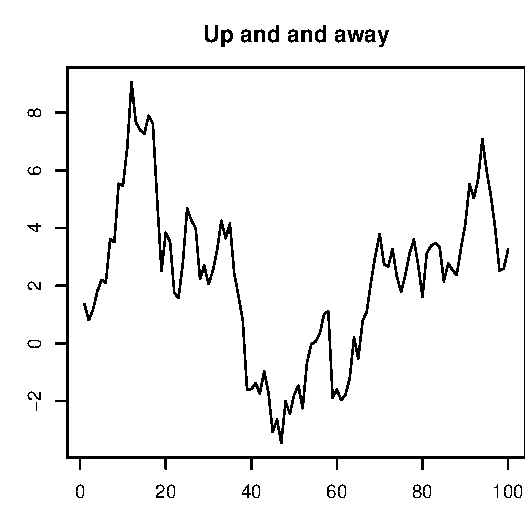
\includegraphics{pinp_files/figure-latex/unnamed-chunk-2-1} \end{center}

The full model had a median \(R^2\) of 0.35, which was higher than the
median \(R^2\) of both the selected and simple models. However, as the
full model had predictors that violated assumptions, it is an
inappropriate multiple regression model so we must take this result with
a grain of salt. The higher \(R^2\) is likely to do with the fact that
the larger number of predictors used would result in overfitting of the
data, and artificially increasing the \(R^2\) even though the
relationship between the wine quality and some of the predictors may not
have been linear in the first place. In comparison, the median \(R^2\)
of our model was 0.32, which was higher than that of the simple model
which was 0.23. Interestingly, as the \(R^2\) of our selected model on
the training data was very similar to the \(R^2\) during in-sample
performance, it appears that our selected model didn't suffer from
overfitting.

Again, discounting the full model, the selected model had the lowest
median MAE 0.527 and RMSE (0.671) of the models being compared,
indicating that it performed better on the testing set of red wine
quality compared to the simple model. (figure name)

\hypertarget{assumption-re-validation}{%
\subsection{\texorpdfstring{\texttt{Assumption\ Re-Validation}}{Assumption Re-Validation}}\label{assumption-re-validation}}

Additionally, our multiple regression model was also checked against the
key assumptions outlined previously -- normality and residual
homoscedasticity. The following figures show that there is no obvious
fanning pattern in the residuals, indicating homoscedasticity, and that
the residuals of the full model are also normally distributed.

\begin{center}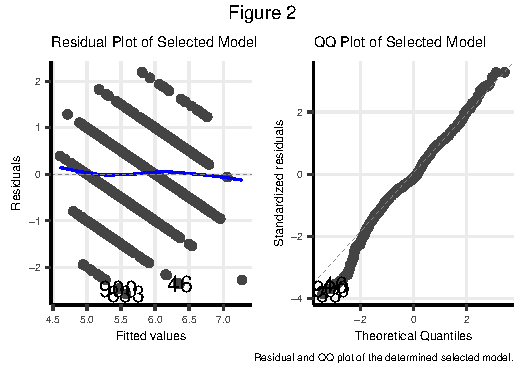
\includegraphics{pinp_files/figure-latex/unnamed-chunk-3-1} \end{center}

\hypertarget{limitations}{%
\subsection{\texorpdfstring{\texttt{Limitations}}{Limitations}}\label{limitations}}

However, this model has a few limitations. The linearity of most
predictor variables against red wine quality, even after attempting
transformations, wasn't very clear and so we had to be generous when
determining what met this assumption for the purpose of analysis. An
\(R^2\) of 0.32 for the selected model is fairly low, which indicates
that the in-sample performance of the model isn't particularly strong,
even though it appears the model didn't run into overfitting issues when
performing 10-fold cross-validation

There is also not much information available on the data collection
process, so we are unsure about whether the different observations are
independent or not. For example, red wines from neighbouring regions may
not be independent and the quality of wine could be influenced as such.
This is an assumption we have had to make for the purpose of the
analysis.

\hypertarget{conclusion}{%
\section{Conclusion}\label{conclusion}}

Overall, we were able to model the quality of red wine by linear
regression, using alcohol concentration, volatile acidity, log of total
sulfur dioxide, and density.

This model could be useful for wine distilleries as any pursuit of
improving the quality of their red wines would be more data-driven,
allowing them to deliberately modify certain characteristics such as
alcohol concentration or total sulphur dioxide in order to achieve a
desired level of quality at a given price point.

\pagebreak

\hypertarget{appendix}{%
\section{Appendix}\label{appendix}}

\begin{center}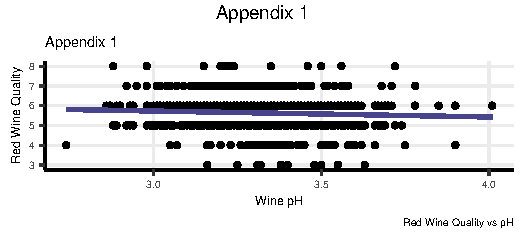
\includegraphics{pinp_files/figure-latex/unnamed-chunk-4-1} \end{center}

\begin{center}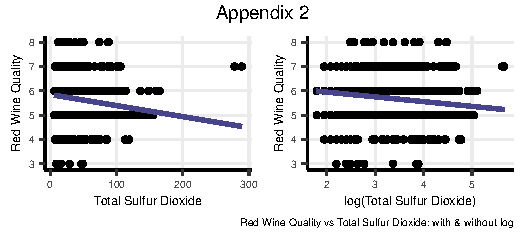
\includegraphics{pinp_files/figure-latex/unnamed-chunk-4-2} \end{center}

\begin{center}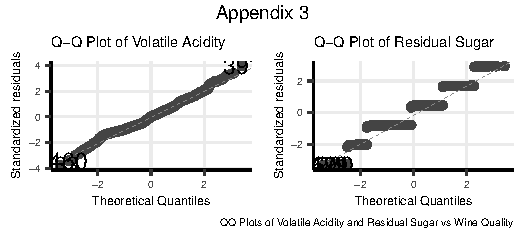
\includegraphics{pinp_files/figure-latex/unnamed-chunk-4-3} \end{center}

\begin{center}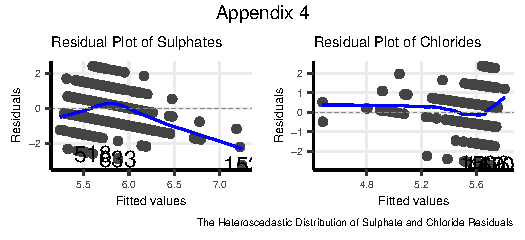
\includegraphics{pinp_files/figure-latex/unnamed-chunk-4-4} \end{center}

%\showmatmethods




\begin{thebibliography}{3}
\newcommand{\enquote}[1]{``#1''}
\providecommand{\natexlab}[1]{#1}
\providecommand{\url}[1]{\texttt{#1}}
\providecommand{\urlprefix}{URL }
\expandafter\ifx\csname urlstyle\endcsname\relax
  \providecommand{\doi}[1]{doi:\discretionary{}{}{}#1}\else
  \providecommand{\doi}{doi:\discretionary{}{}{}\begingroup
  \urlstyle{rm}\Url}\fi
\providecommand{\eprint}[2][]{\url{#2}}

\bibitem[{Allaire \emph{et~al}(2017)Allaire, {R Foundation}, Wickham, {Journal
  of Statistical Software}, Xie, Vaidyanathan, {Association for Computing
  Machinery}, Boettiger, {Elsevier}, Broman, Mueller, Quast, Pruim, Marwick,
  Wickham, Keyes, and Yu}]{CRAN:rticles}
Allaire J, {R Foundation}, Wickham H, {Journal of Statistical Software}, Xie Y,
  Vaidyanathan R, {Association for Computing Machinery}, Boettiger C,
  {Elsevier}, Broman K, Mueller K, Quast B, Pruim R, Marwick B, Wickham C,
  Keyes O, Yu M (2017).
\newblock \emph{rticles: Article Formats for R Markdown}.
\newblock R package version 0.4.1,
  \urlprefix\url{https://CRAN.R-project.org/package=rticles}.

\bibitem[{MacFarlane J (2017)}]{pandoc}
MacFarlane J (2017).
\newblock \emph{Pandoc: A Universal Document Converter}.
\newblock Version 1.19.2.1, \urlprefix\url{http://pandoc.org}.

\bibitem[{Xie Y (2017)}]{}
Xie Y (2017).
\newblock \emph{knitr: A General-Purpose Package for Dynamic Report Generation
  in R}.
\newblock R package version 1.17, \urlprefix\url{https://yihui.name/knitr/}.

\bibitem[{Wickham et al., (2019)}]{}
Wickham et al., (2019).
\newblock \emph{Welcome to the tidyverse. Journal of Open
Source Software, 4(43), 1686}.
\newblock \urlprefix\url{https://doi.org/10.21105/joss.01686}.

\bibitem[{McLean MW(2017)}]{}
McLean MW (2017).
\newblock \emph{RefManageR: Import and Manage BibTeX and BibLaTeX
References in R. The Journal of Open Source Software}.
\newblock \urlprefix\url{https://doi.org/10.21105/joss.00338}.

\bibitem[{McLean MW (2014)}]{}
McLean MW (2014).
\newblock \emph{Straightforward Bibliography Management in R
Using the RefManager Package. arXiv: 1403.2036 [cs.DL]{}}.
\newblock \urlprefix\url{https://arxiv.org/abs/1403.2036}.

\bibitem[{Schloerke B, Cook D, Larmarange J, Briatte F,
Marbach M, Thoen E, Elberg T and Crowley J (2021)}]{}
Schloerke B, Cook D, Larmarange J, Briatte F,
Marbach M, Thoen E, Elberg T and Crowley J (2021).
\newblock \emph{GGally: Extension to ggplot2}.
\newblock R package version 2.1.2. \urlprefix\url{https://CRAN.R-project.org/package=GGally}.

\bibitem[{Fox J and Weisberg S (2019)}]{}
Fox J and Weisberg S (2019).
\newblock \emph{R Companion to Applied
Regression, Third Edition. Thousand Oaks CA: Sage}.
\newblock \urlprefix\url{https://socialsciences.mcmaster.ca/jfox/Books/Companion/}.

\bibitem[{Tang Y, Horijoshi M and Li W (2016)}]{}
Tang Y, Horijoshi M and Li W (2016)
\newblock \emph{ggfortify: Unified
Interface to Visualize Statistical Result of Popular R Packages}.
\newblock The R Journal 8.2 (2016): 478-489.

\bibitem[{Lüdecke D (2021)}]{}
Lüdecke D (2021)
\newblock \emph{sjPlot: Data Visualization for Statistics in
Social Science}.
\newblock R package version 2.8.9 \urlprefix\url{https://CRAN.R-project.org/package=sjPlot}.

\bibitem[{Anderson D, Heiss A, Sumners J (2021)}]{}
Anderson D, Heiss A, Sumners J (2021).
\newblock \emph{equatiomatic: Transform Models into LaTeX Equations}.
\newblock R package version 0.3.0 \urlprefix\url{https://CRAN.R-project.org/package=equatiomatic}.

\bibitem[{Faraway J (2016)}]{}
Faraway J (2016).
\newblock \emph{faraway: Functions and Datasets for Books}.
\newblock R package version 1.0.7 \urlprefix\url{https://CRAN.R-project.org/package=faraway}.

\bibitem[{Broman K(2015)}]{}
Broman K (2015).
\newblock \emph{R/qtlcharts: interactive graphics for
quantitative trait locus mapping}.
\newblock \urlprefix\url{doi:10.1534/genetics.114.172742}.

\bibitem[{Kuhn M (2021)}]{}
Kuhn M (2021).
\newblock \emph{caret: Classification and Regression Training}.
\newblock R package version 6.0-90. \urlprefix\url{https://CRAN.R-project.org/package=caret}.

\bibitem[{Zhu H (2021)}]{}
Zhu H (2021).
\newblock \emph{ableExtra: Construct Complex Table with 'kable' and Pipe Syntax}.
\newblock R package version 1.3.4. \urlprefix\url{https://CRAN.R-project.org/package=kableExtra}..

\bibitem[{Firke S (2021)}]{}
Firke S (2021).
\newblock \emph{Janitor: Simple Tools for Examining and Cleaning Dirty Data}.
\newblock R package version 2.1.0. \urlprefix\url{https://CRAN.R-project.org/package=janitor}.

\bibitem[{Wickham H, François R, Henry L and Müller K (2021)}]{}
Wickham H, François R, Henry L and Müller K (2021).
\newblock \emph{dplyr: A Grammar of Data Manipulation}.
\newblock R package version 1.0.7. \urlprefix\url{https://CRAN.R-project.org/package=dplyr}.

\bibitem[{Lumley T(2020)}]{}
Lumley T(2020).
\newblock \emph{leaps: Regression Subset Selection}.
\newblock  R package version 3.1.0. \urlprefix\url{https://CRAN.R-project.org/package=leaps}.

\bibitem[{Tarr G (2021)}]{}
Tarr G (2021).
\newblock \emph{Week three Lecture L08: Testing for independence – who was more likely to die on the Titanic?}.
\newblock [Powerpoint Slides]. DATA2002, University of Sydney, Sydney, Australia. 

\bibitem[{Tarr G (2021)}]{}
Tarr G (2021).
\newblock \emph{Week eleven Lecture L26: Simple linear regression}.
\newblock [Powerpoint Slides]. DATA2002, University of Sydney, Sydney, Australia. 

\bibitem[{Tarr G (2021)}]{}
Tarr G (2021).
\newblock \emph{Week eleven Lecture L27: Multiple regression and model selection}.
\newblock [Powerpoint Slides]. DATA2002, University of Sydney, Sydney, Australia. 

\bibitem[{Tarr G (2021)}]{}
Tarr G (2021).
\newblock \emph{Week eleven Lecture L28: Prediction internals and performance assessment}.
\newblock [Powerpoint Slides]. DATA2002, University of Sydney, Sydney, Australia. 

\bibitem[{Tarr G (2021)}]{}
Tarr G (2021).
\newblock \emph{Week ten Live Lecture}.
\newblock [Video file]. DATA2002, University of Sydney, Sydney, Australia. 

\bibitem[{Tarr G (2021)}]{}
Tarr G (2021).
\newblock \emph{Week eleven Live Lecture}.
\newblock [Video file]. DATA2002, University of Sydney, Sydney, Australia. 

\bibitem[{Winemakers Academy (2013)}]{}
Winemakers Academy (2013).
\newblock \emph{Understanding Wine Acidity}.
\newblock \urlprefix\url{https://winemakersacademy.com/understanding-wine-acidity/}.

\bibitem[{Alekseeva D (N.D.)}]{}
Alekseeva D (N.D.).
\newblock \emph{Red and White Wine Quality}.
\newblock \urlprefix\url{https://rstudio-pubs-static.s3.amazonaws.com/57835_c4ace81da9dc45438ad0c286bcbb4224.html#:~:text=1%20%2D%20fixed%20acidity%3A%20most%20acids,to%20an%20unpleasant%2C%20vinegar%20taste}.

\bibitem[{Winemakers Academy (2013)}]{}
Winemakers Academy (2013).
\newblock \emph{Understanding Wine Acidity}.
\newblock \urlprefix\url{https://winemakersacademy.com/understanding-wine-acidity/}.

\bibitem[{The Beverage People (2021)}]{}
The Beverage People (2021).
\newblock \emph{How To Use and Test Free SO2 in Wine}.
\newblock \urlprefix\url{https://www.thebeveragepeople.com/how-to/wine/free-so2-in-wine.html}.

\bibitem[{Vinny Dr. (2009)}]{}
Vinny Dr. (2009).
\newblock \emph{What do "pH" and "TA" numbers mean to a wine?}.
\newblock \urlprefix\url{https://www.winespectator.com/articles/what-do-ph-and-ta-numbers-mean-to-a-wine-5035}.

\bibitem[{Slinkard S (2021)}]{}
Slinkard S (2021).
\newblock \emph{Understanding Wine Sulfites}.
\newblock \urlprefix\url{https://www.thespruceeats.com/what-are-wine-sulfites-3511277}.

\bibitem[{Iowa State University (2018)}]{}
Iowa State University (2018).
\newblock \emph{Total Sulfur Dioxide – Why it Matters, Too!}.
\newblock \urlprefix\url{https://www.extension.iastate.edu/wine/total-sulfur-dioxide-why-it-matters-too/}.

\end{thebibliography}

\end{document}
